\documentclass{article}
\setlength{\parindent}{0ex}
\setlength{\parskip}{1em}
\usepackage[utf8]{inputenc} 
\usepackage{amsfonts}
\usepackage{amsmath}
\usepackage{amsthm}
\renewenvironment{proof}[1][\proofname]{{\bfseries #1.}}{\qed}
\usepackage{amssymb}
\usepackage{amstext}
\usepackage{fancybox}
\usepackage{tikz}
\usepackage{tkz-euclide}
\usepackage{gensymb}
\usepackage{graphicx}
\usepackage{verbatim}
\usepackage{qtree}
\usepackage{scrextend}
\usepackage{multirow}
\usepackage{float}
\usepackage{algpseudocode}
\usepackage[bottom]{footmisc}
\usepackage[toc,page]{appendix}

\tikzset{main node/.style={circle,fill=blue!20,draw,minimum size=1cm,inner sep=0pt},
}


%Kodestyling \begin{lstlisting}
\usepackage{color}
\usepackage{listings}
\lstset{ %
language=C++,                % choose the language of the code
%basicstyle=\footnotesize,       % the size of the fonts that are used for the code
basicstyle=\ttfamily,
numbers=left,                   % where to put the line-numbers
numberstyle=\footnotesize,      % the size of the fonts that are used for the line-numbers
stepnumber=1,                   % the step between two line-numbers. If it is 1 each line will be numbered
numbersep=5pt,                  % how far the line-numbers are from the code
backgroundcolor=\color{white},  % choose the background color. You must add \usepackage{color}
showspaces=false,               % show spaces adding particular underscores
showstringspaces=false,         % underline spaces within strings
showtabs=false,                 % show tabs within strings adding particular underscores
frame=single,           % adds a frame around the code
tabsize=2,          % sets default tabsize to 2 spaces
captionpos=b,           % sets the caption-position to bottom
breaklines=true,        % sets automatic line breaking
breakatwhitespace=false,    % sets if automatic breaks should only happen at whitespace
escapeinside={\%*}{*)},          % if you want to add a comment within your code
mathescape
}

\usepackage{caption}
\captionsetup[table]{name=Tabel}

\usepackage{mathtools}
\DeclarePairedDelimiter\ceil{\lceil}{\rceil}
\DeclarePairedDelimiter\floor{\lfloor}{\rfloor}


\def\meta#1{\mbox{$\langle\hbox{#1}\rangle$}}
\def\macrowitharg#1#2{{\tt\string#1\bra\meta{#2}\ket}}

{\escapechar-1 \xdef\bra{\string\{}\xdef\ket{\string\}}}

\def\intro#1{{#1}{\cal I}}
\def\elim#1{{#1}{\cal E}}

\showboxbreadth 999
\showboxdepth 999
\tracingoutput 1


\let\imp\to
\def\elim#1{{{#1}{\cal E}}}
\def\intro#1{{{#1}{\cal I}}}
\def\lt{<}
\def\eqdef{=}
\def\eps{\mathrel{\epsilon}}
\def\biimplies{\leftrightarrow}
\def\flt#1{\mathrel{{#1}^\flat}}
\def\setof#1{{\left\{{#1}\right\}}}
\let\implies\to
\def\KK{{\mathsf K}}
\let\squashmuskip\relax

\graphicspath{ {images/} }
\usetikzlibrary{arrows}
\tikzset{
  leaf_/.style = {shape=rectangle,draw, align=center},
  node_/.style     = {shape=circle,draw,align=center}
}
\author{Rune Kok Nielsen (qkd362), Andreas Holm (jnh508)}
\title{GraphHopper kernel in C++}
\DeclareMathOperator{\Ran}{Ran}
\DeclareMathOperator{\Dom}{Dom}

\renewcommand*\contentsname{Indholdsfortegnelse}
\begin{document}
	
\maketitle
\newpage
\tableofcontents
\newpage

\section{Introduction}

\section{SVM (Short summary)}
\subsection{Kernels}

\section{GraphHopper}
The following description of the GraphHopper kernel is based on the presentation in \cite{graphhopper}.

GraphHopper is a graph kernel, i.e. a kernel for comparing graph data. The kernel effectively analyses the structure of the graphs by comparing subtrees similarly to the \textit{shortest path kernel}\footnote{We introduce the shortest path kernel in our earlier work \cite{svm-graph-kernels}.} (SPK). An advantage of these kernels is that they may analyse not only the structure of the graphs but also the attributes of their nodes.
While SPK compares all shortest paths with a complexity of $\mathcal{O}(n^4)$, where $n$ is the number of nodes, GraphHopper only compares shortest paths of equal length with complexity $\mathcal{O}(n^2(m+\log n+\delta^2 + d))$ where $m$ is the number of edges, $\delta$ is the diameter of the graph and $d$ is the dimension of the node attributes. The complexity will be explained along with the algorithm itself.

Let $G=(V,E)$ and $G'=(V',E')$ be graphs such that $V,V'$ are nodes and $E,E'$ are edges and let $P,P'$ be the sets of all shortest paths in $G$ and $G'$ respectively. The kernel is then a sum of path kernel $k_p$ over each pair of shortest paths $\pi\in P,\ \pi'\in P'$:

\begin{equation}
\label{eq:k}
k_{graphhopper}(G,G')=\sum_{\pi\in P}\sum_{\pi'\in P'}k_p(\pi, \pi')
\end{equation}
The path kernel $k_p$ is a sum of some node kernel $k_n$ on each pair of nodes $v\in\pi,\ v'\in\pi'$ such that $v$ and $v'$ appears at the same place in $\pi$ and $\pi'$ for pairs $\pi$ and $\pi'$ of equal discrete length\footnote{Discrete length meaning that $\pi$ and $\pi'$ contains the same number of nodes.}. I.e.
\begin{equation}
\label{eq:k_p}
k_p(\pi, \pi')=\begin{cases}
\sum_{i=1}^{|\pi|}k_n(\pi(i), \pi'(i)) & \text{for }|\pi|=|\pi'|\\
0 & \text{otherwise}
\end{cases}
\end{equation}
where $\pi(i)$ denotes the $i$'th node in $\pi$. The node kernels that we have chosen to implement are all described in a later section and are not essential in describing the kernel itself.

Using the definition above we now present a simple example. Consider the two graphs, $G$ and $G'$ in figure \ref{fig:shortest-path-graph}.


\begin{figure}[H]
	\begin{minipage}[t]{0.7\linewidth}
		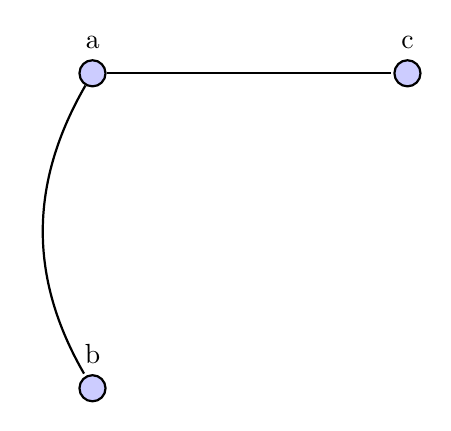
\begin{tikzpicture}[-,>=stealth',shorten >=1pt,auto,node distance=4cm,
		thick,main node/.style={circle,fill=blue!20,draw,font=\sffamily\Large\bfseries}]
		
		\node[main node] (a) [label=a] {};
		\node[main node] (b) [below of=a, label=b] {};
		\node[main node] (c) [right of=a, label=c] {};
		
		
		\path[every node/.style={font=\sffamily\small}]
		(a) edge [bend right] node {}(b)
		(a) edge node {}(c)
		;
		\end{tikzpicture}
	\end{minipage}
	\begin{minipage}[t]{0.2\linewidth}
		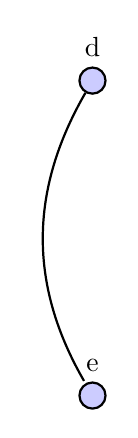
\begin{tikzpicture}[-,>=stealth',shorten >=1pt,auto,node distance=4cm,
		thick,main node/.style={circle,fill=blue!20,draw,font=\sffamily\Large\bfseries}]
		
		
		\node[main node] (d) [label=d] {};
		\node[main node] (e) [below of=d, label=e] {};
		
		
		\path[every node/.style={font=\sffamily\small}]
		(d) edge [bend right] node {}(e)
		;
		\end{tikzpicture}
	\end{minipage}
	\caption{\textit{Left: G. Right: G'}}
	\label{fig:shortest-path-graph}
\end{figure}
Identifying shortest paths we get
\begin{align*}
P&=\{[a], [a,b], [a,c], [b], [b,a], [b,a,c], [c], [c,a], [c,a,b]\}\\
P'&=\{[d],[d,e],[e],[e,d]\}
\end{align*}
We can now compute $k_{graphhopper}$ by summing over all paths $\pi\in P$ and $\pi'\in P'$ such that $|\pi|=|\pi'|$. E.g. the pair $\pi=[a]\in P,\ \pi'=[d]\in P'$ are of equal discrete length so we add $k_n(a, d)$ to the sum. Identifying more pairs we find, for instance, that $|\pi|=|\pi'|$ for $\pi=[a,b]\in P,\ \pi'=[d,e]\in P'$ so we add $k_n(a,d) + k_n(b, e)$. For completeness of the example the entire sum can be seen in (\ref{eq:example_sum}).

\begin{equation}
\label{eq:example_sum}
\begin{split}
k_{graphhopper}(G,G')	&=  k_n(a,d) + k_n(a, e) + (k_n(a, d) + k_n(b, e)) + (k_n(a, e) + k_n(b, d)) \\ 
				&+ (k_n(a, d) + k_n(c, e)) + (k_n(a, e) + k_n(c, d)) + k_n(b, d) + k_n(b, e) \\
				&+ (k_n(b, d) + k_n(a, e)) + (k_n(b, e) + k_n(a, d)) + k_n(c, d) + k_n(c, e) \\
				&+ (k_n(c, d) + k_n(c, e)) + (k_n(c, e) + k_n(a, d))
\end{split}
\end{equation}

Observe how we added $k_n(a,d)$ multiple times to the final sum. Naturally, the number of times $k_n(v, v')$ will be added (where $v\in V,\ v'\in V'$) will be exactly the number of pairs of paths $\pi\in P,\ \pi'\in P'$ such that $|\pi|=|\pi'|$ and $\pi(i)=v,\ \pi'(i)=v'$ for some $i$.

Let $w(v, v')$ be the number of times we have to add $k_n(v, v')$ for some pair $v\in V,\ v'\in V'$ as described above. Instead of computing and adding $k_n(v, v')$ repeatedly we may instead add $w(v,v') k_n(v, v')$ once. We call $w(v, v')$ the $\textit{weight}$ between the two nodes and rewrite the kernel as a weighted sum between pairs of nodes:
\begin{equation}
k_{graphhopper}(G,G')=\sum_{v\in V}\sum_{v'\in V'}w(v,v')k_n(v,v')
\end{equation}


When calculating $w(v,v')$ we sum the number of pairs $\pi,\pi'$ such that $|\pi|=|\pi'|$ and $\pi(i)=\pi'(i)$ for some $i$. Let $width(G)$ be the discrete length of the longest shortest path $\pi\in P$ and let $\delta=min(width(G), width(G'))$. Since we only consider pairs of paths of same length and the longest shortest path we do not have to consider any paths of length greater than $\delta$.

\iffalse
\begin{proof}[Proof: We may ignore paths of length greather than $\delta$]\\
Consider any two graphs $G,\ G'$ such that $width(G)=\delta$. Then we either have $\delta=width(G')$ or $\delta<width(G')$.\\
Let $width(G)=\delta=width(G')$ and let $\pi'\in P'$ such that $|\pi'|>\delta$. Since $G'$ is at least as wide as any shortest paths within it we have $width(G')\geq |\pi'|>\delta = width(G')$ which is an absurdity.\\
Let $width(G)=\delta < width(G')$ and let $\pi'\in P'$ such that $|\pi'|>\delta$. Now assume that there exists some $\pi\in P$ such that $|\pi|=|\pi'|$. We now see that $width(G)\geq |\pi| = |\pi'|>\delta=width(G)$ which is an absurdity.\\
We have now proven that there can not exist any pairs of paths $\pi\in P,\ \pi'\in P'$ such that $|\pi|=|\pi'|>\delta$.
\end{proof}
\fi

Beside from this limitation it is trivial that for a pair of paths $\pi,\ \pi'$ such that $|\pi|=|\pi'|=j$ we only have to consider nodes at index $i=1..j$ since there cannot exist any nodes at index $i>j$.


We can now formalize $w(v,v')$ as
\begin{equation}
w(v,v')=\sum_{j=1}^{\delta}\sum_{i=1}^{j}|\{(\pi, \pi')\ |\ \pi(i)=v,\ \pi'(i)=v',\ |\pi|=|\pi'|=j\}|
\end{equation}


Let $\delta=width(G)$ and let $M$ be a $|V|\times\delta\times\delta$ matrix such that $M(v)_{ij}$ is the number of shortest paths $\pi\in P$ such that $|\pi|=j$ and $\pi(i)=v$. We then have
\begin{equation}
w(v,v')=\sum_{j=1}^{\delta}\sum_{i=1}^{j}M(v)_{ij}*M'(v')_{ij}
\end{equation}
allowing us to easily find the weight between pairs of nodes by first computing $M$ and $M'$. Furthermore, when computing $K$ for multiple graphs we may compute all M matrices beforehand and use them in the pairwise computations instead of computing them for each pair of graphs.


\subsection{Computing $M$}
The $M$ matrix can be computed in a number of ways. We will be using the message-passing algorithms presented in \cite{graphhopper}

Let $\tilde{v}$ be a node in $V$ and let $P_{\tilde{v}}$ be the set of shortest paths in $G$ starting in $\tilde{v}$. Then $M(v)_{ij}$ becomes $\sum_{\tilde{v}\in V}$ number of times $v$ appears as the $i$'th node in each $\pi_{\tilde{v}}\in P_{\tilde{v}}$ of discrete length $j$. This means that we can compute $M$ by iterating over each node $\tilde{v}\in V$ and finding all shortest paths starting in $\tilde{v}$.

Before we move on, we will first introduce the shortest path DAG $G_{\tilde{v}}=(V, E_{\tilde{v}})$ for $\tilde{v}$ where $E_{\tilde{v}}$ are edges kept in $G_{\tilde{v}}$. The shortest path DAG $G_{\tilde{v}}$ is created by removing a minimum amount of edges from $G$ so that it only contains edges that are part of some shortest path starting in $\tilde{v}$. We call $\tilde{v}$ the root node in the resulting DAG. This is illustrated in figure \ref{fig:shortest-path-dag} where we present a graph $G$ and the shortest path DAG $G_{a}$ rooted in $a$.

\begin{figure}[H]
	\begin{minipage}[t]{0.7\linewidth}
		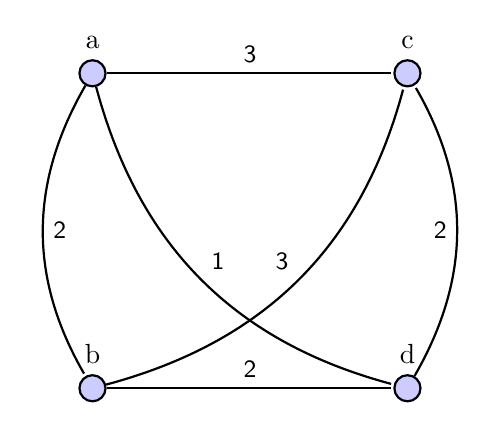
\begin{tikzpicture}[-,>=stealth',shorten >=1pt,auto,node distance=4cm,
		thick,main node/.style={circle,fill=blue!20,draw,font=\sffamily\Large\bfseries}]
		
		\node[main node] (a) [label=a] {};
		\node[main node] (b) [below of=a, label=b] {};
		\node[main node] (c) [right of=a, label=c] {};
		\node[main node] (d) [below of=c, label=d] {};
		
		
		\path[every node/.style={font=\sffamily\small}]
		(a) edge [bend right] node {2}(b)
		(a) edge node {3}(c)
		(a) edge [bend right] node {1}(d)
		(d) edge [bend right] node {2}(c)
		(b) edge node {2}(d)
		(b) edge [bend right] node {3}(c)
		;
		\end{tikzpicture}
	\end{minipage}
	\begin{minipage}[t]{0.2\linewidth}
		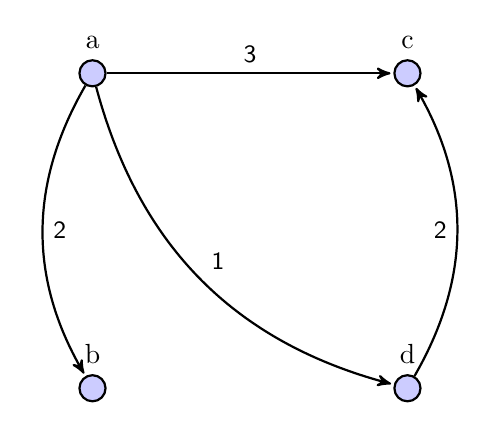
\begin{tikzpicture}[->,>=stealth',shorten >=1pt,auto,node distance=4cm,
		thick,main node/.style={circle,fill=blue!20,draw,font=\sffamily\Large\bfseries}]
		
		
		\node[main node] (a) [label=a] {};
		\node[main node] (b) [below of=a, label=b] {};
		\node[main node] (c) [right of=a, label=c] {};
		\node[main node] (d) [below of=c, label=d] {};
		
		
		\path[every node/.style={font=\sffamily\small}]
		(a) edge [bend right] node {2}(b)
		(a) edge node {3}(c)
		(a) edge [bend right] node {1}(d)
		(d) edge [bend right] node {2}(c)
		;
		\end{tikzpicture}
	\end{minipage}
	\caption{\textit{Left: G. Right: $G_{\tilde{a}}$}}
	\label{fig:shortest-path-dag}
\end{figure}

We now introduce two more constructs used for computing $M$: $\mathfrak{O}_{\tilde{v}}$ and $\mathfrak{D}_{\tilde{v}}$. 

\subsubsection{Computing $\mathfrak{O}_{\tilde{v}}$}
Let $\mathfrak{O}_{\tilde{v}}$ be a $n\times\delta$ matrix where $\mathfrak{O}_{\tilde{v}}(v,i)$ is the number of paths from $\tilde{v}$ to $v$ in the shortest path DAG $G_{\tilde{v}}$ with discrete length $i$.

\textbf{Example}\\
Using the graph illustrated in figure \ref{fig:shortest-path-dag}, we find that there are two paths from $a$ to $c$ in $G_{\tilde{a}}$ of discrete length 2 and 3 so $\mathfrak{O}_{a}(c,1)=0,\ \mathfrak{O}_{a}(c,2)=1,\ \mathfrak{O}_{a}(c,3)=1$.

The rows of $\mathfrak{O}_{\tilde{v}}$, denoted by $\mathfrak{o}_{\tilde{v}}^v$, are computed recursively using a message-passing algorithm starting at the root. Intuitively, there is always exactly one path from the root to itself in the shortest path DAG and this path is of discrete length 1 so $\mathfrak{o}_{\tilde{v}}^{\tilde{v}}=[1]$. From the current node, the algorithm passes a message to each of its reachable neighbours (children) containing its own row shifted one place to the right and adds the contents to the child's row. The algorithm then repeats on the next level of nodes. This is illustrated in figure \ref{fig:compute_o}.


\begin{figure}[H]
	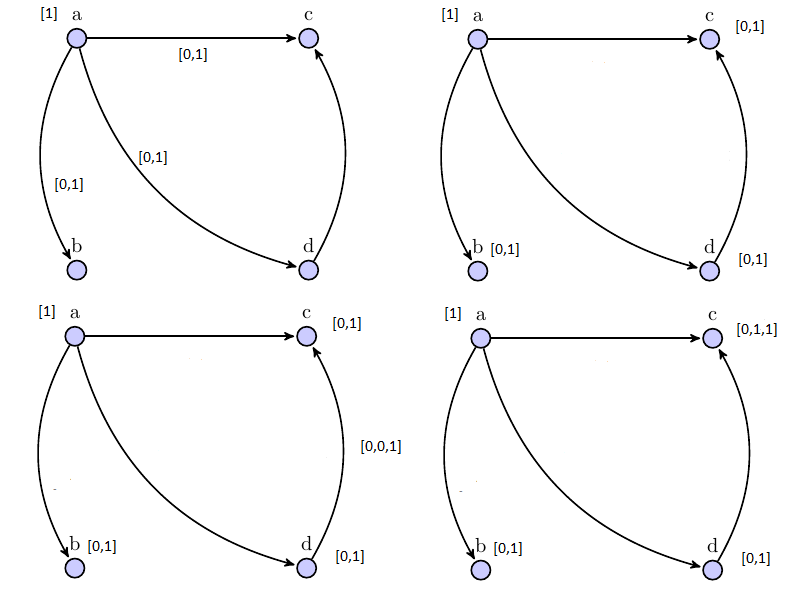
\includegraphics[width=12cm]{compute_o}
	\caption{\textit{Computing $\mathfrak{O}_{\tilde{a}}$ using message-passing. Detailed in appendix \ref{appendix:illustrations_compute_o}.}}
	\label{fig:compute_o}
\end{figure}


Before defining the algorithm for computing $\mathfrak{O}_{\tilde{v}}$ we must define two constructs. First, let $\oplus$ be left-aligned addition between two vectors such that their length is aligned. I.e.:
\begin{equation}
[a, b] \oplus [c, d, e] = [a + c, b + d, e]
\end{equation}
Now, let $V_{\tilde{v}}^j$ be the nodes in $G_{\tilde{v}}$ such that there exists some path from the root to $v$ in $G_{\tilde{v}}$ with discrete length $j$. The algorithm is shown in figure \ref{algorithm:o}.

\begin{figure}[H]
\begin{lstlisting}
$\mathfrak{o}_{\tilde{v}}^{\tilde{v}}=[1]$
$\mathfrak{o}_{\tilde{v}}^v=[0], for\ v\in V \ {\tilde{v}}$
for $j=1..\delta$
   for $v\in V_{\tilde{V}}^j$
      for $w$ in $v$.children
         $\mathfrak{o}_{\tilde{v}}^w=\mathfrak{o}_{\tilde{v}}^w\oplus[0,\mathfrak{o}_{\tilde{v}}^v]$
      end
   end
end
\end{lstlisting}
\caption{Algorithm for computing $\mathfrak{O}_{\tilde{v}}$}
\label{algorithm:o}
\end{figure}

When computing $\mathfrak{O}_{\tilde{v}}$ each node sends exactly one message of size $\leq \delta$ to all of its children which are then updated. I.e. $|E_{\tilde{v}}|$ messages of size $\leq \delta$ giving a complexity of $\mathcal{O}(|E_{\tilde{v}}|\delta) \leq \mathcal{O}(|E|\delta)$.

\subsubsection{Computing $\mathfrak{D}_{\tilde{v}}$}

Let $\mathfrak{D}_{\tilde{v}}$ be a $n\times\delta$ matrix where $\mathfrak{D}_{\tilde{v}}(v, i)$ is the number of paths of discrete length $i$ in $G_{\tilde{v}}$ starting in $v$.

\textbf{Example}\\
Consider the node $d$ in figure \ref{fig:shortest-path-dag}. From this node there is one path in $G_{\tilde{a}}$ to itself of discrete length 1 ($\pi_1=[d]$) and one path to $c$ of discrete length 2 ($\pi_2=[d,c]$) so $\mathfrak{D}_a(d,1)=1,\ \mathfrak{D}_a(d,2)=1,\ \mathfrak{D}_a(d,i)=0$ for $i\notin\{1,2\}$.

The algorithm for computing $\mathfrak{D}_{\tilde{v}}$ will, like in the case of $\mathfrak{O}_{\tilde{v}}$, be using a message-passing approach. In this case the row for node $v$ in $\mathfrak{D}_{\tilde{v}}$ is denoted by $\mathfrak{d}_{\tilde{v}}^v$. We start by observing that all nodes must have exactly one path of discrete length 1 (the path to themselves) so we initialize $\mathfrak{d}_{\tilde{v}}^v=[1],\ \forall v\in V$. The $\mathfrak{d}_{\tilde{v}}^v$ row for $v$ is then computed by adding (using the $\oplus$ operation defined earlier) the rows of its children shifted one place to the right. The rows of the children are computed recursively until a leaf node is reached and the result is then send up through the stack of recursive calls. This is illustrated in figure \ref{fig:compute_d}.
\begin{figure}[H]
	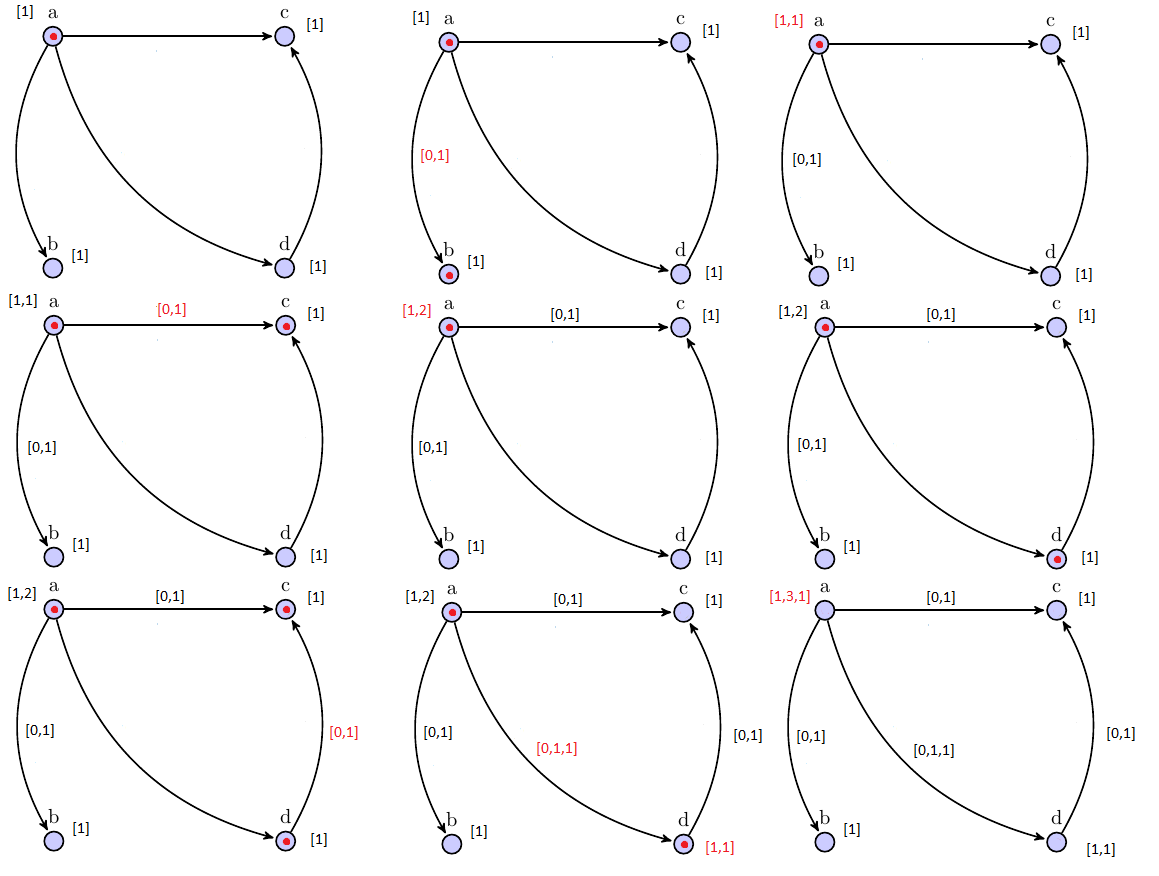
\includegraphics[width=12cm]{compute_d}
	\caption{\textit{Computing $\mathfrak{d}_{\tilde{a}}$ using message-passing.  Detailed in appendix \ref{appendix:illustrations_compute_d}.}}
	\label{fig:compute_d}
\end{figure}

A recursive algorithm for computing $\mathfrak{D}_{\tilde{v}}$ can then be written out as in figure \ref{algorithm:d}.

\begin{figure}[H]
\begin{lstlisting}
function compute_d_rec(v)
   if not $\mathfrak{d}_{\tilde{v}}^v$.is_computed
      for $w$ in $v$.children
         $\mathfrak{d}_{\tilde{v}}^v = \mathfrak{d}_{\tilde{v}}^v \oplus $[0,compute_d_rec(w)]
      end
      $\mathfrak{d}_{\tilde{v}}^v$.is_computed = true
   end
   return $\mathfrak{d}_{\tilde{v}}^v$
end
	
initialize: $\mathfrak{d}_{\tilde{v}}^v=[1],\ \forall v\in V$
compute_d_rec($\tilde{v}$)
	
\end{lstlisting}
	\caption{Algorithm for computing $\mathfrak{D}_{\tilde{v}}$}
	\label{algorithm:d}
\end{figure}

When computing $\mathfrak{D}_{\tilde{v}}$ with the algorithm detailed in figure \ref{algorithm:d} a node visits each of its children in $G_{\tilde{v}}$ exactly once when computing its row and in this process their rows are computed recursively. Effectively, each edge $e\in E_{\tilde{v}}$ will be traversed once and each time a message will be returned of size $\leq \delta$ which updates the calling node. This gives a complexity of $\mathcal{O}(|E_{\tilde{v}}|\delta)\leq(|E|\delta)$


\subsubsection{Putting things together}
Having computed $\mathfrak{O}_{\tilde{v}}$ and $\mathfrak{D}_{\tilde{v}}$ we now observe that the number of times that $v$ appears as the $i$'th node in a path of discrete length $j$ in $G_{\tilde{v}}$ must be the number of paths from $\tilde{v}$ to $v$ in $G_{\tilde{v}}$ of length $i$ times the number of paths of length $j-i+1$ in $G_{\tilde{v}}$ starting in $v$; i.e. $\mathfrak{O}_{\tilde{v}}^v(v,i)\mathfrak{D}_{\tilde{v}}(v,j - i + 1)$.

\textbf{Example}\\
Consider the node $d$ in figure \ref{fig:shortest-path-dag}. Trying to find the number of paths in $G_{a}$ such that $d$ is the 2nd node in a path of length 3 we can intuitively see that there is one such path: $[a,d,c]$. This equivalent to the number of paths of length 2 from $a$ to $d$ times the number of paths of length $3-2+1=2$ starting in $d$.
This could be computed using the $\mathfrak{o}_a^d$ and $\mathfrak{d}_a^d$ computed earlier in figures \ref{fig:compute_o} and \ref{fig:compute_d}:
\begin{align}
\mathfrak{o}_a^d(2)\mathfrak{d}_a^d(3-2+1)&=\mathfrak{o}_a^d(2)\mathfrak{d}_a^d(2)\\
&=1 * 1\\
&=1
\end{align}

Being able to efficiently count the number of times $v$ appears as the $i$'th node in a path of length $j$ in a shortest path from $\tilde{v}$ we can now look back at the definition of $M(v)$ and conclude that

\begin{equation}
M(v)_{ij} = \sum_{\tilde{v}\in V}\mathfrak{o}_{\tilde{v}}^v(i)\mathfrak{d}_{\tilde{v}}^v(j-i+1)
\end{equation}

Computing $M$ may be achieved using the algorithm shown in figure \ref{alg:compute_M}. First we compute $G_{\tilde{v}},\mathfrak{O}_{\tilde{v}},\mathfrak{D}_{\tilde{v}}$ for all $\tilde{v}\in V$. Using a Dijkstra implementation with complexity $\mathcal{O}(m\log n)$\footnote{Using a binary-heap implementation as described in \cite{alg-bible} and assuming that all nodes are reachable.} to compute $G_{\tilde{v}}$ this gives a complexity of $\mathcal{O}(n((m\log n) + m\delta + m\delta)) = \mathcal{O}(n((m\log n + m\delta))$. We then iterate over each pair of $v,\tilde{v}$ and $j=1..\delta,i=1..j$ giving a complexity of $\mathcal{O}(n^2\delta^2)$. Adding this together we get a total complexity of
\begin{align}
\mathcal{O}(n(m\log n + m\delta) + n^2\delta^2)&=\mathcal{O}(n(m\log n + m\delta + n\delta^2))\\
\end{align}

\begin{figure}[H]
\begin{lstlisting}
for $\tilde{v}\in V$
   compute $G_{\tilde{v}}$ using Dijkstra
   compute $\mathfrak{O}_{\tilde{v}}$
   compute $\mathfrak{D}_{\tilde{v}}$
end
let $M$ be a $n\times \delta \times \delta$ matrix of zeros
for $v \in V$
   for $\tilde{v}\in V$ 
      for $j\in 1..\delta$
         for $i\in 1..j$
            $M(v)_{ij}+=\mathfrak{o}_{\tilde{v}}^v(i)\mathfrak{d}_{\tilde{v}}^v(j-i+1)$
         end
      end
   end
end
\end{lstlisting}
\caption{Algorithm for computing M.}
\label{alg:compute_M}
\end{figure}

\subsection{Computational analysis}
To compute $k_{graphopper}$ we sum over each pair of nodes which, given precomputed $w(v,v')$ and $k_n(v,v')$, gives a complexity of $\mathcal{O}(n^2)$. Assuming that the complexity of computing $k_n(v,v')$ grows linearly relative to the dimension $d$ of the node attributes the complexity of computing all $k_n(v,v')$ has a complexity of $\mathcal{O}(n^2d)$. Computing $w(v,v')$ consists of summing for $j\leq \delta,i\leq j$ giving $\mathcal{O}(\delta^2)$ and doing this for each pair gives a complexity of $\mathcal{O}(n^2\delta^2)$. Together this gives a complexity of $\mathcal{O}(n^2(d + \delta^2))$. Before doing these computations, however, we must compute the $M$ matrices as described earlier adding up to a total runtime of
\begin{align}
&\mathcal{O}(n^2(d + \delta^2) + n(m\log n + m\delta + n\delta^2))\\
=\ &\mathcal{O}(n^2(d+\delta^2)+nm(\log n + \delta))
\end{align}


\subsection{Implementation}
In this section we present the algorithm used in our implementation of GraphHopper described using pseudo-code. Based on the theory explained earlier we are able to effectively split the computation into two steps:
\begin{enumerate}
	\item Compute $M$ for all graphs.
	\item Compute $K$ using all pairs of M.
\end{enumerate}
The code presented here will not be a 1:1 match with the actual implementation but rather an introduction to the algorithm. We will exclude unneeded details including optimizations that are not required to understand the implementation.

\subsubsection{Computing M}

\begin{lstlisting}
#Computes the M matrix for a graph
function computeM($graph$){
   for $\tilde{v}\in graph.V$
      prepareNode($\tilde{v}$)
   end
   
   #Let M be an $|V|\times\delta\times\delta$ array of zeros
   $graph.M$ = array$[|graph.V|][graph.\delta][graph.\delta]$
   #Now sum the data of $\mathfrak{D}$ and $\mathfrak{O}$
   for $v\in graph.V$
      for $\tilde{v}\in graph.V$
         for $j\in 1..graph.\delta$
            for $i\in 1..j$
               $M[v][i][j] += \mathfrak{o}_{\tilde{v}}^v(i)\mathfrak{d}_{\tilde{v}}^v(j-i+1)$
            end
         end
      end
   end
}

#Computes $\mathfrak{O}_{\tilde{v}}$ and $\mathfrak{D}_{\tilde{v}}$
#Starts by creating $G_{\tilde{v}}$ using Dijkstra 
#before computing the matrices.
function prepareNode($graph$, $\tilde{v}$)
   #Prepare data for Dijkstra
   $queue = []$
   for $v\in graph.V$
      $v.d = \infty$
      $v.parents = []$
      $v.children = []$
      $queue.append(v)$
   end
   $\tilde{v}.d = 0$
   #$queue$ is a min heap allowing us to pop
   #the node with lowest d
   $queue.make\_min\_heap()$
   $\delta = 0$
   while not $queue.empty()$
      $u = queue.front()$
      $queue.pop()$
      
      $d = u.d + 1$
      for $v \in u.adjacent$
         if $v.d \geq d$
            if $v.d > d$
               $v.parents = []$
            end
            $v.parents.append(u)$
            $v.d = d$
            $\delta=max(\delta, d)$
         end
      end
      $queue.make\_min\_heap()$
   end
   #Set the graph's width to be the maximum width
   #found computing Dijkstra for any $\tilde{v}$
   $graph.\delta = max(graph.\delta, \delta)$
   
   #Putting nodes in buckets grouped and ordered
   #by shortest distance to $\tilde{v}$
   $\tilde{v}.ordered = $group_nodes($graph.V$)
   
   #Use $parents$ data to define $children$ in nodes
   prepare_children($graph.V$)
   
   #Refer to algorithms in last theory section
   computeO($\tilde{v},\ \delta$)
   computeD($\tilde{v}$)
end


\end{lstlisting}

\subsection{Gaps}
The following section is based on the description of GraphHopper with gaps from \cite{gappy}

Some of the graphs we are using are extracted from images, and because they are extracted from images they can contains errors, in form of missing edges, this can occur because the process of extracting graphs from images is not perfect. To minimize the impact of these error we can choose to apply gaps in our paths, this will minimize the impact of the errors mentioned earlier, because the new paths will close some of the gaps, where there might be missing edges. In figure \ref{fig:simple_gaps} is it shown how we can apply these new paths to a simple graph.

\begin{figure}[H]
	\begin{minipage}[t]{0.7\linewidth}
		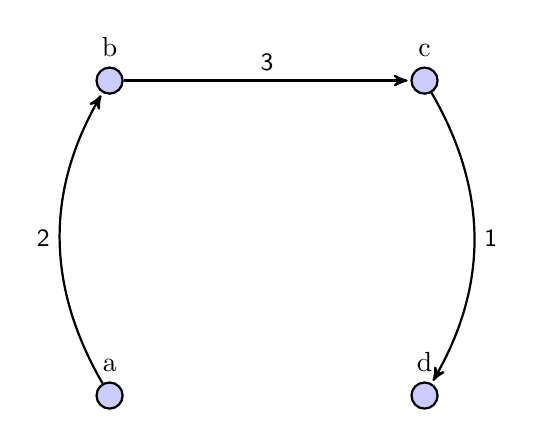
\begin{tikzpicture}[->,>=stealth',shorten >=1pt,auto,node distance=4cm,
		thick,main node/.style={circle,fill=blue!20,draw,font=\sffamily\Large\bfseries}]
		
		
		\node[main node] (b) [label=b] {};
		\node[main node] (a) [below of=b, label=a] {};
		\node[main node] (c) [right of=b, label=c] {};
		\node[main node] (d) [below of=c, label=d] {};
		
		
		\path[every node/.style={font=\sffamily\small}]
		(a) edge [bend left] node {2}(b)
		(b) edge node {3}(c)
		(c) edge [bend left] node {1}(d)
		;
		\end{tikzpicture}
	\end{minipage}
	\begin{minipage}[t]{0.2\linewidth}
		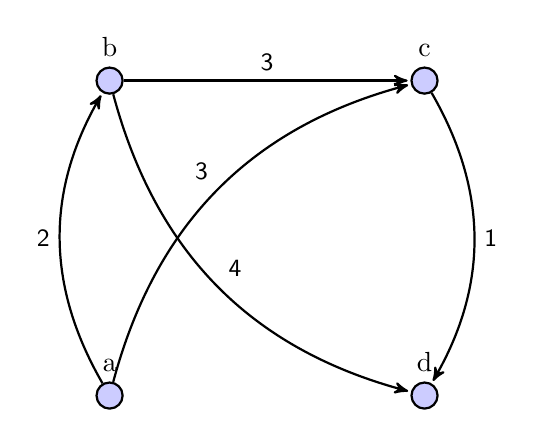
\begin{tikzpicture}[->,>=stealth',shorten >=1pt,auto,node distance=4cm,
		thick,main node/.style={circle,fill=blue!20,draw,font=\sffamily\Large\bfseries}]
		
		
		\node[main node] (b) [label=b] {};
		\node[main node] (a) [below of=b, label=a] {};
		\node[main node] (c) [right of=b, label=c] {};
		\node[main node] (d) [below of=c, label=d] {};
		
		
		\path[every node/.style={font=\sffamily\small}]
		(a) edge [bend left] node {2}(b)
		(b) edge node {3}(c)
		(c) edge [bend left] node {1}(d)
		(a) edge [bend left] node {3}(c)
		(b) edge [bend right] node {4}(d)
		;
		\end{tikzpicture}
	\end{minipage}
	\caption{\textit{Left: Without gaps. Right: With gaps of size 1.}}
	\label{fig:simple_gaps}
\end{figure}
In figure \ref{fig:simple_gaps} we apply new paths with a gap size of $1$, in figure X we show how we can increase the gap size, and insert paths that skip up to $s$ amount of nodes.


When we apply gaps to our graphs, we do not need to change our graph kernel in anyway, we can simply use our already established $k_{graphhopper}$ graph kernel.


\subsubsection{Implementation}
In this section we will show how simple it is to add gaps to our current graphhopper implementation.

\begin{lstlisting}
function prepareNode($graph$, $\tilde{v}$)
# Before


end


\end{lstlisting}

\section{Node kernels}
\subsection{Dirac}
Dirac in GraphHopper simply compare the 2 given nodes, to see if they are equal to each other, and if they are equal we return $1$, and if they are not equal we return $0$. This kernel is primarily used when we compare graphs that contain discrete node labels, and the node labels are discrete and does not represent a continuous value. 
This node kernels can only be used when we compare graphs with discrete node labels. The node kernel can be seen formally described in (\ref{eq:dirac}), where $x$ and $x'$ are the given node labels.
\begin{equation}
\label{eq:dirac}
k_{dirac}(x, x')=\begin{cases}
1 & \text{for }x=x'\\
0 & \text{otherwise}
\end{cases}
\end{equation}

\subsection{Linear}
The linear node kernel is the dot product of $x$ and $x'$, it can be seen formally described in (\ref{eq:linear}).
\begin{equation}
\label{eq:linear}
k_{linear}(x, x') = x(i) \cdot x'(i)
\end{equation}

In figure X it is show how our linear kernel behave when comparing discrete node values.

\subsection{Gaussian}
For our gaussian kernel we are using a simplified version of (\ref{eq:gaussian}), this will save  us time when we are calculating \textit{K}, our simplified version can be seen in (\ref{eq:gaussian_simple}) where $\mu = \frac{1}{2 \sigma^2}$, these two formulas will yield the same result, but when we use (\ref{eq:gaussian_simple}) we save time by eliminating some operations, because we are doing them beforehand, and this speeds up the process of calculating $K$.
\begin{equation}
\label{eq:gaussian}
k_{gaussian}(x, x') = exp(-\frac{||x - x'||^2}{2\sigma^2})
\end{equation}
\begin{equation}
\label{eq:gaussian_simple}
k_{gaussian}(x, x') = exp(-\mu ||x - x'||^2)
\end{equation}
We are using our gaussian kernel when we are comparing graphs where the node label either consist of a vector or discrete values which represent a continuous value.

To show how the gaussian kernel behave when comparing discrete node values, we have drawn a graph, which can be seen in figure X, it is easy to see that the graph is growing exponentially the less the difference between $x$ and $y$ is.

\subsection{Bridge}
Our bridge kernel is based on \cite{shortest-path} bridge formula, but because we are working with vectors, we subtract the vectors and then normalize them, instead of just subtracting them. The bridge formula can be seen in (\ref{eq:bridge}).
\begin{equation}
\label{eq:bridge}
k_{bridge}(x, x') = \text{max}(0, c - |(||x - x'||)|)
\end{equation}

The bridge's behaviour can be compared to the gaussian's behaviour, but instead of growing exponentially it grows linearly, and declines linearly. 

\subsection{Dirac times Gaussian}
\begin{equation}
\label{eq:diractimesgaussian}
k_{diractimesgaussian}(x, x') = k_{dirac}(x, x') k_{gaussian}(x, x')
\end{equation}

\section{Product}

\section{Experiments}
\subsection{Runtime experiments (C++ vs MATLAB)}
\subsubsection{Results}

System specs
\begin{table}[H]
	\centering
	\hspace*{-0.7in}
	\scalebox{0.7} {
		\begin{tabular}{c|c|c|c}
			ID & OS & CPU & Ram\\
			\hline
			A & Win7 64 bit & Intel i5-3320M @ 2.60GHz (4 cores) & 8GB \\
			\hline
			B & Win10 64 bit & AMD FX-8150 Black Edition @ 3.60GHz (8 cores) & 16GB
			
		\end{tabular}
	}
	\caption{\textit{System specs}}
	\label{table:specs}
\end{table}


Runtime in seconds for calculating $K$ (without gaps).
\begin{table}[H]
	\centering
	\hspace*{-0.7in}
	\scalebox{0.7} {
		\begin{tabular}{c|c|c|c|c|c}
			Data set & Node kernel & Runtime in MATLAB & Runtime in Mex C++ & System spec & Ratio\\
			\hline
			Mutag & Dirac & 31.6 & \textbf{0.731} & A & 1:43.23\\
			Enzymes & Dirac & 722.99 & \textbf{16.9} & A & 1:42.78\\
			Enzymes (Symmetrized) & Gaussian & 256.14 & \textbf{26.55} & A & 1:9.65 \\ 
			Airways subsampled & Gaussian & 5518.01 & \textbf{2608.45} & A & 1:2.12
			
		\end{tabular}
	}
	\caption{\textit{Runtime results}}
	\label{table:runtime_results}
\end{table}

\subsubsection{Discussion}
\subsection{Accuracy experiments (Gaps vs. no Gaps)}

\subsubsection{Results}

\begin{table}[H]
	\centering
	\hspace*{-0.7in}
	\scalebox{0.7} {
		\begin{tabular}{c|c|c|c}
		Data set & Node kernel & Without gaps & With gaps (size 1)\\
		\hline
		Mutag & Dirac & $\mathbf{83.111 (std. 1.9633)}$ & $79.000 (std. 2.2801)$\\
		Enzymes & Dirac & $\mathbf{35.133 (std. 2.050)}$ & $\mathbf{36.350 (std. 1.3888)}$\\
		Enzymes (symmetrized) & Gaussian & $\mathbf{67.850 (std. 1.3482)}$ & $\mathbf{67.250 (std. 1.5138)}$\\
		Airways subsampled & Gaussian & $\mathbf{63.180 (std. 1.7900)}$ & $\mathbf{62.600 (std. 1.3233)}$
		\end{tabular}
	}
	\caption{\textit{Accuracy results}}
	\label{table:raccuracy_results}
\end{table}

\subsubsection{Discussion}

\section{Conclusion}





\iffalse
\section{The GraphHopper kernel}
Description of kernel as 


\section{Restructuring the kernel}
In order to take advantage of the strengths of C++ we first have to restructure the kernel to achieve a new calculation based on sums as opposed to matrix operations.

In \cite{graphhopper} the weight between two nodes $v$ and $v'$ are given by
\begin{equation}
w(v,v')=\sum_{j=1}^{\delta}\sum_{i=1}^{\delta}\sharp\{(\pi, \pi')|\pi(i)=v,\pi'(i)=v',|\pi|=|\pi'|=j\}=\langle M(v),M(v')\rangle
\end{equation}
where $(M(v))_{ij}$ is the number of times that $v$ appears as the $i^{th}$ node in a shortest path in $G$ of discrete length $j$. As described in the last section (CITATION) this amounts to $\sum_{\tilde{v}\in V}\mathfrak{D}_{\tilde{v}}(v,j-i+1)\mathfrak{O}_{\tilde{v}}(v,i) = \sum_{\tilde{v}\in V}(\mathfrak{d}_{\tilde{v}}^v)_{j-i+1}(\mathfrak{o}_{\tilde{v}}^v)_i$.

Using these definitions of $(M(v))_{ij}$ we see that
\begin{align}
w(v,v')&=\sum_{j=1}^{\delta}\sum_{i=1}^{\delta}\sharp\{(\pi, \pi')|\pi(i)=v,\pi'(i)=v',|\pi|=|\pi'|=j\}\\
&=\sum_{j=1}^{\delta}\sum_{i=1}^{\delta}(M(v))_{ij}(M(v'))_{ij}\\
&=\sum_{j=1}^{\delta}\sum_{i=1}^{\delta}\left(\sum_{\tilde{v}\in V}(\mathfrak{d}_{\tilde{v}}^v)_{j-i+1}(\mathfrak{o}_{\tilde{v}}^v)_i\right)\left(\sum_{\tilde{v'}\in V'}(\mathfrak{d}_{\tilde{v'}}^{v'})_{j-i+1}(\mathfrak{o}_{\tilde{v'}}^{v'})_i\right)
\end{align}
showing that we can calculate the weights using only the row vectors of $\mathfrak{D}$ and $\mathfrak{O}$ which can be computed using message passing as described in algorithms 1 and 3 in \cite{graphhopper} given the shortest path DAG's for $G$ and $G'$.

Further, since we do not need to eqaute the left hand equation to the product of two matrices and since $i\leq j$ for any $\pi$ such that $|\pi|=j$ and $\pi(i)$ exists we only need to sum for $i\leq j$:

\begin{equation}
w(v,v')=\sum_{j=1}^{\delta}\sum_{i=1}^{j}\left(\sum_{\tilde{v}\in V}(\mathfrak{d}_{\tilde{v}}^v)_{j-i+1}(\mathfrak{o}_{\tilde{v}}^v)_i\right)\left(\sum_{\tilde{v'}\in V'}(\mathfrak{d}_{\tilde{v'}}^{v'})_{j-i+1}(\mathfrak{o}_{\tilde{v'}}^{v'})_i\right)
\end{equation}
\fi


\newpage

\renewcommand\refname{References}
\begin{thebibliography}{9}
		\bibitem{graphhopper}
		Aasa Feragen, Niklas Kasenburg, Jens Petersen, Marleen de Bruijne, Karsten M. Borgwardt.
		\emph{Scalable kernels for graphs with continuos attributes}.
		In Advances in Neural Information Processing Systems, pages 216-224, 2013.

		\bibitem{gappy}
		Aasa Feragen, Karsten Borgwardt.
		\emph{Efficient tree-path kernels for attributde trees}.
		2013.

		\bibitem{shortest-path}
		Karsten M. Borgwardt, Hans-Peter Kriegel.
		\emph{Shortest-path kernels on graphs}.
		In Proceedings of the International Conference on Data Mining, pages 74-81, 2005.
		
		\bibitem{svm-graph-kernels}
		Rune Kok Nielsen, Andreas Holm.
		\emph{Afløsningsopgave i fagområdet Modellering og Analyse af Data}.
		University of Copenhagen, 2016\\
		https://drive.google.com/file/d/0BxPtSV8mme0xWGV0ZlpKRlFUU0U/view
		
		\bibitem{alg-bible}
		Thomas H. Cormen, Charles E. Lesierson, Ronald L. Rivest, Clifford Stein.
		\emph{Introduction to Algorithms 3rd ed.}.
		MIT Press, 2009.
		
\end{thebibliography}


\newpage
\begin{appendices}
\section{Illustration comments}
\label{appendix:illustrations}
This section serves to explain the details of illustrations used in the report itself that may not be self-explanatory.
\subsection{Figure \ref{fig:compute_o}}
\label{appendix:illustrations_compute_o}
Reading left to right, top to bottom, the steps are as follows:
\begin{enumerate}
	\item The root sends a message to its children.
	\item The children's values are updated.
	\item The only non-leaf node in the next level is $d$, so it sends a message to its only child, $c$.
	\item The value of $c$ is updated. The only node in the next level is $c$, which is a leaf node, so the algorithm ends.
\end{enumerate}


\subsection{Figure \ref{fig:compute_d}}
\label{appendix:illustrations_compute_d}
Reading left to right, top to bottom, the steps are as follows:
\begin{enumerate}
	\item The algorithm starts at the root node $a$.
	\item The node $a$ asks $b$. Since $b$ is a leaf node it does not need to do any further work so it returns $[0, 1]$.
	\item The result from $b$ is added to $a$: $[1] \oplus [0,1] = [1,1]$.
	\item The node $a$ asks $c$. Like $b$, $c$ is a leaf node and returns $[0,1]$.
	\item The result is added to $a$: $[1,1] \oplus [0,1] = [1,2]$.
	\item The node $a$ asks $d$. Since $d$ is not a leaf node it must first determine its own value before returning.
	\item The node $d$ asks $c$ which returns $[0,1]$.
	\item The result from $c$ is added to $d$: $[1] \oplus [0,1] = [1,1]$ and $d$ returns $[0,1,1]$.
	\item The result from $d$ is added to $a$: $[1,2]\oplus[0,1,1]=[1,3,1]$. The root node has now collected the values of all its children so the algorithm ends.
\end{enumerate}
\end{appendices}

\end{document}